\documentclass[11pt]{article}


\usepackage[letterpaper,bindingoffset=0.2in,
            left=1in,right=1in,top=1in,bottom=1in,
            footskip=.25in]{geometry}
\usepackage{hyperref}
	\hypersetup{
			colorlinks=true,
			linkcolor=black,
			filecolor=magenta,      
			urlcolor=blue,
	}
\usepackage{graphicx}
	\graphicspath{ {images/} }
\usepackage{listings}
\usepackage{fancybox}
\usepackage{subfig}
\usepackage[justification=centering]{caption}
\usepackage[section]{placeins}


% Code to center a listing
% https://tex.stackexchange.com/questions/85489/how-to-center-a-lstlisting
\makeatletter
\newenvironment{CenteredBox}{% 
\begin{Sbox}}{% Save the content in a box
\end{Sbox}\centerline{\parbox{\wd\@Sbox}{\TheSbox}}}% And output it centered
\makeatother

	
\begin{document}


\title{COMP SCI 5401 FS2017 Assignment 2c}
\author{Stuart Miller\\\href{mailto:sm67c@mst.edu}{sm67c@mst.edu}}
\maketitle


\section{Overview}\label{sect:overview}

Assignment 2c provides an improvement to the Iterative Prisoner's Dilemma (IPD) problem by employing a coevolutionary Genetic Programming Search across single agents evaluated by a tit-for-tat strategy. 


\section{Methodology}\label{sect:methodology}
As before, the algorithm works by generating a population of random trees (50\% full depth trees, 50\% grown tress), then iteratively generating children based on tree crossover from parents. Children are occasionally mutated, then simulated by playing tit-for-tat to obtain a fitness rating and added to the population. To obtain this fitness rating, each agents is plays a set number of rounds on a tit-for-tat strategy (the agent's opponent chooses what the agent itself did last). An option is also present to score each agent's fitness across multiple runs of IPD, with multiple randomized initial memories. Doing so allows for a more accurate fitness rating. After each generation, the population is thinned by removing poor agents chosen in a k-tournament. 

The main feature of this solution involves computing not only an absolute fitness for each agent, but also a composite coevolutionary fitness. This fitness is calculated after each generation is established (i.e. after all children have had their fitness independently evaluated). This composite fitness (referred to as "comp\_fitness" or variables prefixed with "comp" in code) is obtained by choosing a random sample of opponents from the population. Opponents are chosen without replacement. The absolute fitnesses of all chosen opponents and the agent itself are averaged and assigned to the agent in question as its composite fitness.

\section{Experimental Setup}\label{sect:exp_setup}

\begin{figure}[ht]
\begin{CenteredBox}
\lstinputlisting[lastline=21,frame=single,linewidth=4in,basicstyle=\small]{../../log/default.txt}
\end{CenteredBox}
\caption{Configuration Values}
\label{fig:config}
\end{figure}

The following default configuration values were chosen (Figure \ref{fig:config}). Some algorithm parameters were dictated in the assignment (d, k, l, seedType, and evals). Termination is set to merely number of evals since this assignment dictated a 10,000 eval minimum. A mu and lambda of 100 and 50 were chosen. This allowed for rather sizable populations, but still a large number of generations before 10,000 evals. A low mutation rate was chosen as GP typically relies more heavily on recombination (this will bee experimentally evaluated later in Section \ref{sect:results}. Survival selection was set to k-Tournaments with a k of 40. This allowed for sufficient exploration. As noted in Section \ref{sect:methodology}, there is an option to re-randomize an agents memory across multiple runs of IPD for more well-rounded fitness. This has been set to 5 here.  Finally, there is a small parsimony coefficient and plus survival strategy. These were simply inherited from the last assignment, since they worked well there.

The variation chosen for this assignment was the mutation operator. I thought it interesting that Koza states that small mutation sizes are preferred for GP, so an examination of this seems appropriate. The three values chosen were 5\%, 0\%, and 80\%. 5\% was the chosen default and seemed like an adequate approximation of Koza's recommended minimal value. 80\% was a sufficiently high number, and 0\% was chosen to see the effect of no mutation at all.

\section{Results}\label{sect:results}
\begin{figure}[ht]
\centering
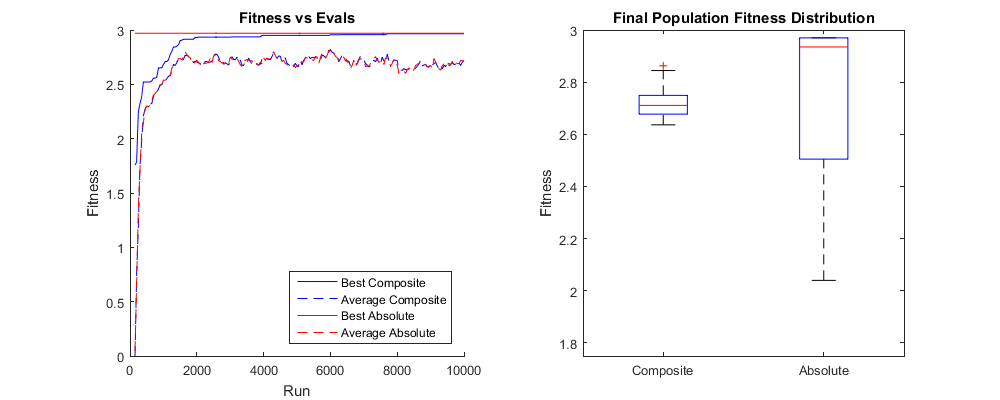
\includegraphics[width=6in]{default.png}
\caption{Default Mutation (5\%) }
\label{fig:graph_default}
\end{figure}

\begin{figure}[ht]
\centering
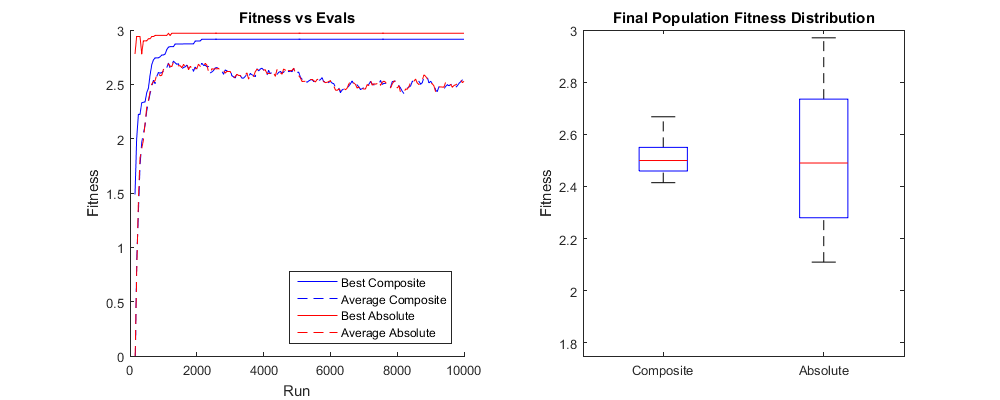
\includegraphics[width=6in]{high_mut.png}
\caption{High Mutation (80\%) }
\label{fig:graph_high_mut}
\end{figure}

\begin{figure}[ht]
\centering
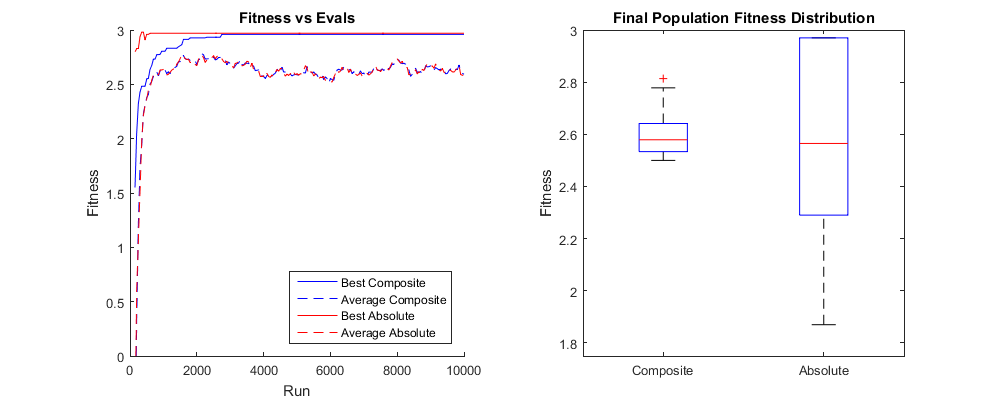
\includegraphics[width=6in]{no_mut.png}
\caption{No Mutation (0\%)}
\label{fig:graph_no_mut}
\end{figure}

\begin{figure}[ht]
\centering
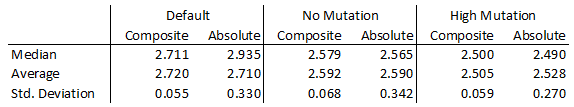
\includegraphics[width=4.5in]{avg_and_std_dev.png}
\caption{Table of Averages}
\label{fig:avg_table}
\end{figure}

\begin{figure}[ht]
\centering
\begin{minipage}{.48\textwidth}
  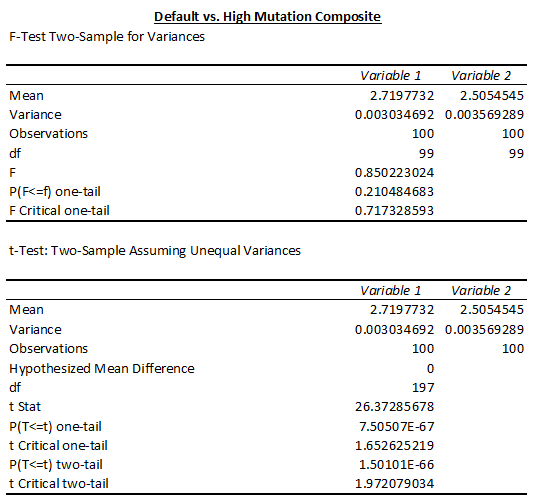
\includegraphics[width=1.0\textwidth]{default_vs_high_comp.png}
  \caption{Default vs. High Mutation \\Composite Fitness}
  \label{fig:default_vs_high_comp}
\end{minipage}\hfill
\begin{minipage}{.48\textwidth}
  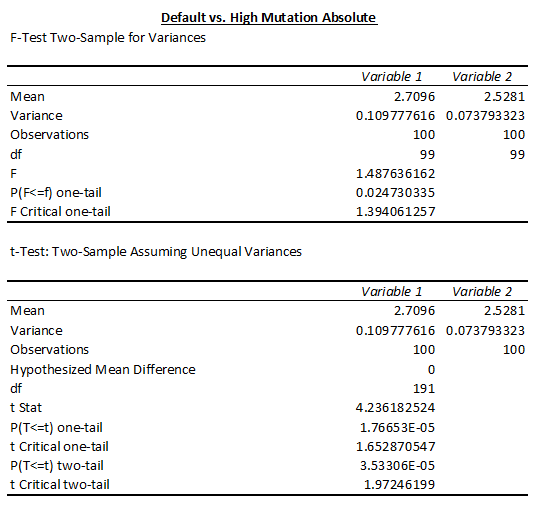
\includegraphics[width=1.0\textwidth]{default_vs_high_abs.png}
  \caption{Default vs. High Mutation \\Absolute Fitness}
  \label{fig:default_vs_high_abs}
\end{minipage}
\end{figure}

\begin{figure}[ht]
\centering
\begin{minipage}{.48\textwidth}
  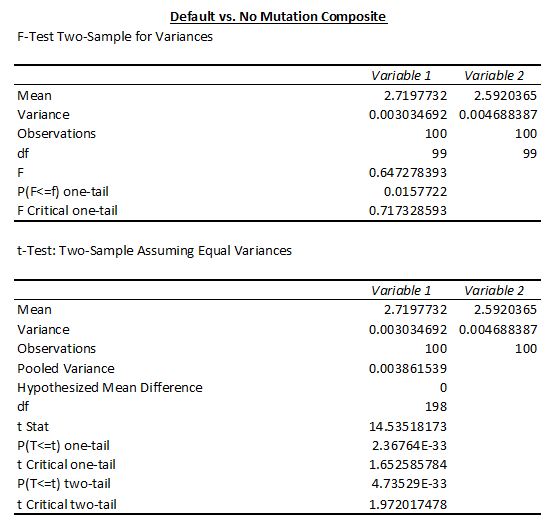
\includegraphics[width=3in]{default_vs_no_comp.png}
  \caption{Default vs. No Mutation \\Composite Fitness}
  \label{fig:default_vs_no_comp}
\end{minipage}\hfill
\begin{minipage}{.48\textwidth}
  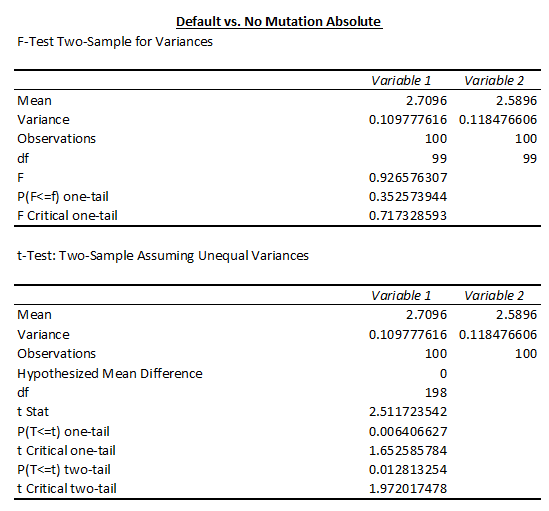
\includegraphics[width=3in]{default_vs_no_abs.png}
  \captionof{figure}{Default vs. No Mutation \\ Absolute Fitness}
  \label{fig:default_vs_no_abs}
\end{minipage}
\end{figure}

\begin{figure}[ht]
\centering
\begin{minipage}{.48\textwidth}
  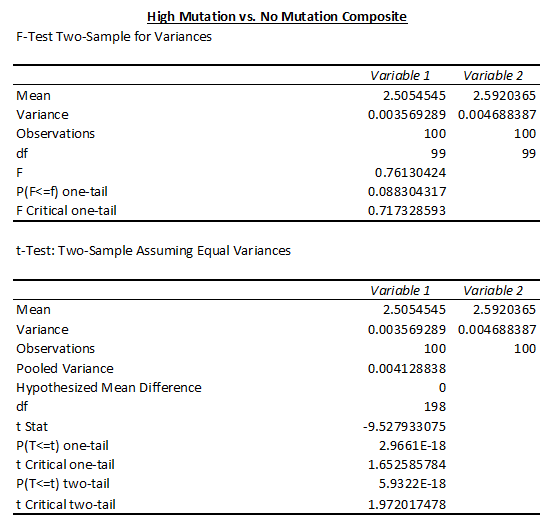
\includegraphics[width=3in]{high_vs_no_comp.png}
  \caption{High Mutation vs. No Mutation \\Composite Fitness}
  \label{fig:high_vs_no_comp}
\end{minipage}\hfill
\begin{minipage}{.48\textwidth}
  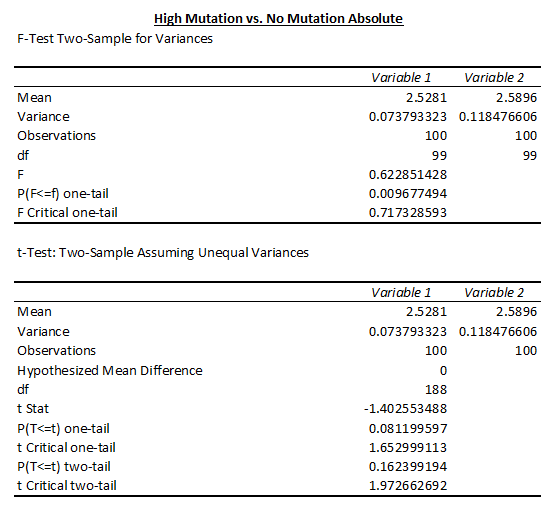
\includegraphics[width=3in]{high_vs_no_abs.png}
  \caption{High Mutation vs. No Mutation \\Absolute Fitness}
  \label{fig:high_vs_no_abs}
\end{minipage}
\end{figure}

\section{Discussion}\label{sect:discussion}

\subsection{Graphical Analysis}\label{sect:graph_anal}
The graphs in Figures \ref{fig:graph_default} - \ref{fig:graph_no_mut} show the best fitnesses in the population over time, split up by composite and absolute fitnesses. It is interesting to note that the average for both fitnesses stays mostly the same whereas the absolute best is always higher. This makes sense as the composite consists of score that is always adjusted lower for its fellow population members.

As for the value of mutation, notice high mutation graph in particular. Its average value actually goes down over time, showing that the excessive exploration is actually hurting it in this instance. Alternatively the fitness vs. evals graphs for no mutation and default mutation are nearly identical.

The really drastic differences become evident in the box plot of the final population. Notice that for default mutation, the red median line is right up near the top, whereas for the high and no mutation, it is in the middle. This is true for both composite and absolute fitnesses, although it is much more pronounced for absolute. (See the table in Figure \ref{fig:avg_table} for the exact numerical values.) In all cases, the default mutation value scored the best fitness (comparing the median and average values of the composite and absolute fitness). This confirms that the default value of a small 5\% mutation rate is preferable.

\subsection{Statistical Analysis}\label{sect:stat_anal}
The statistical analysis can be seen in Figures \ref{fig:default_vs_high_comp} - \ref{fig:high_vs_no_abs}. In all cases except for absolute fitness High Mutation vs. No Mutation, the null hypothesis can be safely rejected, concluding that there is not a statistically proven advantage to using high mutation over no mutation (or vice versa). This is acceptable though, as the main point that the default mutation of 5\% is better still stands true.

\section{Conclusion}\label{sect:conclusion}
It is clear from the analysis in Section \ref{sect:graph_anal} that the default mutation rate of 5\% is most beneficial. This follows with the advice given by Koza and stated in class lectures. It is interesting to note, however, that using no mutation at all is not necessarily better or worse than using too much mutation; each suffer from roughly equivalent decreased performance. 

Additionally, none of the parameters ever allowed the algorithm to attain anything above a 3 payoff. It was relatively easy for the algorithm to settle on a solution where both agents cooperate, but impossible to find an appropriate time to defect. Perhaps this is the most beneficial solution, as, in real-life prisoners dilemna situation, it is much preferable to take the mutually beneficial payout rather than to go for the extreme scenario and risk complete loss.


\end{document}